\documentclass{article}
\usepackage{indentfirst}
\usepackage{latexsym}
\usepackage{bm}
\usepackage{amsmath}
\usepackage{amssymb} 
\usepackage{tikz,mathpazo}
\usetikzlibrary{shapes.geometric, arrows}
\usepackage{flowchart}
\usepackage{subfigure}
\usepackage{hyperref}
\setlength{\parindent}{0em}


\title{Self-calibration in liquid scintillator detectors}  
\author{Dou Wei, Jianfeng Zhou}  
\date{\today}

\begin{document}

\maketitle
\abstract{}
\section{Introduction}
\subsection{Calibration of scintillator detector may bring extra challenges}
\subsubsection{The advantages of scintillator detector}
\par Scintillator is a good candidate for neutrino observation for its better energy resolution and low energy threshold. However, to calibrate a scintillation detector is a hard work.
\subsubsection{Why calibration is so difficult}
\par 1. The calibration source need high purity, which adds high difficulties to the mechanical process and demand high cost. 2. It is hard to fix calibrate source in the detector, which may cause extra accident, either. 3. The structure of the calibration source may bring shadows which is different to the real situation, requiring more correction in simulation.
\subsubsection{The objective of this paper is to reconstruct with no calibration detector}
\par 1.  We try to reconstruct the vertex and unknown structures if we have plenty of data without calibration. 2. If calibration is done, a cross check can be applied to reduce the error in measurement. 
\subsection{The importance of reconstruction}
\subsubsection{Why reconstruction is so important?}
\par Reconstruction is necessary for reduce the background caused by PMT and supporting structures , raise the energy resolution and identify the particle type. 
\subsubsection{Who else has done that?}
\par 1.Traditional reconstruction is a likelihood or divide detectors into many segment bins, such as Daya Bay. (How to reconstruct resolution by Borexino, SNO+, Daya Bay)\\
\par 2. Machine learning has broadly applied in current physical experiments, such as neural networks. 3. EM algorithm is useful in estimating the unknown distribution. and been widely used in many aspects.

\subsection{Highlight of this paper and purpose of this paper}
\par This is the first series reconstruction without calibration. The main algorithm uses EM algorithm to reconstruct vertex and time profile. 	We use software JSAP based on ROOT system and GEANT4. and reconstruction.
\par Section 2 shows the how EM algorithm reconstruct vertex and time profile in different steps. and E-step and M-step is section 2.3.1 and 2.3.2. Section 3 shows the simulation condition and reconstruction result. Section 4 shows the conclusion and discussion.

\section{EM Algorithms for Reconstruction}
\subsection{Using EM iteration to raise the resolution}
\subsubsection{How traditional EM algorithm update parameters}
\par EM is useful in estimate unknown distribution. Each step maximize the likelihood use the parameters in last step.

	\begin{equation}
	\numberwithin{equation}{section}
		\begin{cases}
		E-step: \tau^{[k+1]} = \arg\max_{\tau}L(\tau^{[k]},\Theta^{[k]};n_i, t_i)\\
		M-step:\Theta^{[k+1]} = \arg\max_{\Theta}L(\tau^{[k+1]},\Theta^{[k]}; n_i, t_i)\\
		\end{cases}
	\end{equation}
	
\par We use M-step find the vertex that maximize the likelihood , for E-step, we add a little correction to make the estimation of the time profile more physical. which will be detailed described in subsection 2.1.3
\par A flow chart to describe simplified EM process is shown in figure \ref{fig:1}

\begin{figure}[htbp]
	\centering
	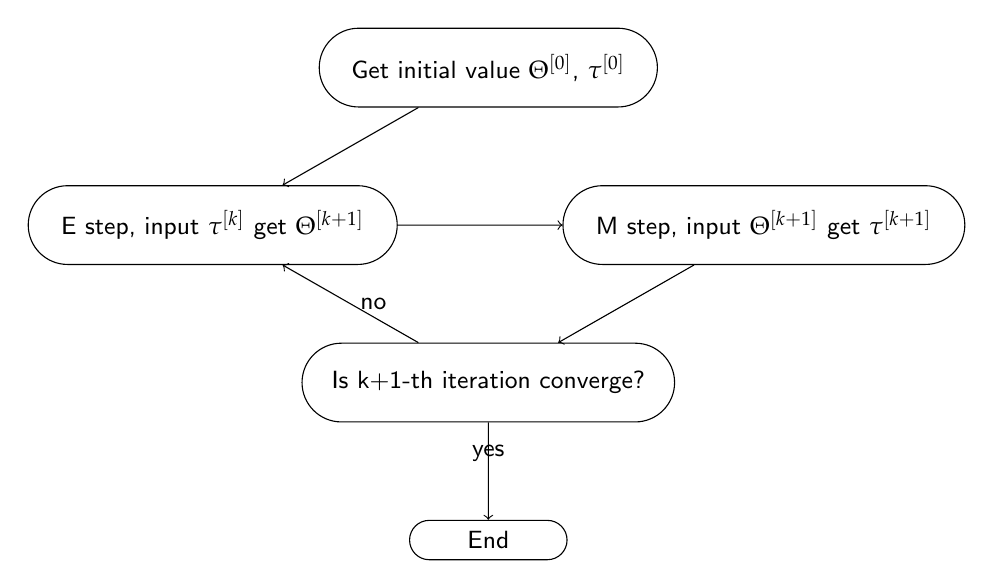
\begin{tikzpicture}[font={\sf \small}]
	\def \smbwd{2cm}

%	\node (step1) at (0,0) [draw, terminal,minimum width=\smbwd, minimum height=0.5cm] {Weighted Average};  
	\node (step2) at (0,-1.5) [draw, terminal,minimum width=\smbwd,minimum height=1cm] {Get initial value $\Theta^{[0]}$, $\tau^{[0]}$}; 
	\node (step3) at (0,-5.5) [draw, terminal, minimum width=\smbwd, minimum height=1cm] {Is k+1-th iteration converge?}; 
	\node (step4) at (-3.5,-3.5) [draw, terminal, minimum width=\smbwd, minimum height=1cm] {E step, input $\tau^{[k]}$ get $\Theta^{[k+1]}$};
	\node (step5) at (3.5,-3.5) [draw, terminal, minimum width=\smbwd, minimum height=1cm] {M step, input $\Theta^{[k+1]}$ get $\tau^{[k+1]}$};
%	\coordinate (point1) at (0,-6.75);
	\node (step6) at (0,-7.5) [draw, terminal,minimum width=\smbwd,minimum height=0.5cm] {End}; 


%	\draw[->] (step1) -- node[right]{$\vec{x}_{col}$} (step2) ;
	\draw[->] (step2) -- node[right]{} (step4);
	\draw[->] (step5) -- node[above]{} (step3);
	\draw[->] (step3) -- node[right]{no} (step4);
	\draw[->] (step4) -- node[right]{}(step5);
	\draw[->] (step3) -- node[above]{yes}(step6);
\end{tikzpicture}
	\caption{The flow chart of the EM reconstruction}
	\label{fig:1}
	
\end{figure}

\subsection{Initial guess of the $\tau_0$ and $\Theta_0$}
\par 1. In 0-th iteration, we first use the pe information to estimate a rough result including the energy and vertex. 
\par 2. Initial guess of vertex and energy. We begin with the vertex using weighted average. 

	\begin{equation}
		\numberwithin{equation}{section}
		\vec{x}_{ini} = \frac{\sum_{i=1}^N n_i\vec{x}_i}{\sum_{i=1}^N n_i}
	\end{equation}

\par 3. Initial guess of  time profile
	Then using the time data reconstruct the time profile by

	\begin{equation}
		\numberwithin{equation}{section}
		p(t) =  \frac{\tau_r+\tau_d}{\tau_d^2} \exp (-\frac{(t-t_0)}{\tau_d})(1-\exp(-\frac{t-t_0}{\tau_r})) (t > t_0)
	\end{equation}

	\begin{equation}
		\numberwithin{equation}{section}
		\tau_d = \arg_{\tau_d}\max{\sum_i \log p_i(t)}
	\end{equation}

\subsection{M-step to find the best fit vertex}
	\par Traditional reconstruction algorithm is applied in M-step. The likelihood function can be resolved into 2 parts
	
	\begin{equation}
		\numberwithin{equation}{section}
		\log L\{\textbf{x},E;n_i,t_j\} = \log L\{\textbf{x},E;n_i\}+\log L\{\textbf{x},E;t_j\}
	\end{equation}
	
	\par  The former part only includes charge information and the latter includes time information readout by photosensors. The likelihood is to calculate the total probability of received photons by each PMT 

	\begin{equation}
	\numberwithin{equation}{section}
	p^*_i =  
		\begin{cases}
 		p_{i,s}\{${\textbf x}$,E\} p_{i,t}\{${\textbf x}$,S(t)\}& \text{$n_i > 0$ (Fired PMT)}\\
 		p_{i,s}\{${\textbf x}$,E\} & \text{$n_i=0$ (Unfired PMT)}
		\end{cases}
	\end{equation}
	
	\begin{equation}
		\numberwithin{equation}{section}
		\log L\{\textbf{x},E\} = \log \prod_{i} p^*_i = 	\sum_{i}\log p_{i,s}\{\textbf{x},E\} +\sum_{i'}\log p_{i',t}\{\textbf{x},S(t)\} 
	\end{equation}
	
	\par $i$ is the index of all PMTs and $i'$ only includes fired PMTs.   
	\par The combined likelihood includes vertex and unknown dependence, which will be reconstructed by maximize the likelihood, and we will derivate detailed form from abstract to a calculative one in the following section.
	
\subsubsection{Spatial-based algorithm based on charge information}
\par The number of photon electrons received by PMT is approximately a Poisson distribution.
	
	\begin{equation}
	\numberwithin{equation}{section}
	p_i = \frac{\xi_i^{n_i}}{n_i!} \exp(-\xi_i)
	\end{equation}
	
	\par To estimate the $\xi_i$, we need to consider the loss on propagation and photo coverage and photo response. The propagation mainly caused by attenuation is nearly an exponential decay. The photo coverage $\Omega_i(\textbf x)$ based on the occupancy of PMTs, while the vertex contributes to the solid angle . Finally, the photo response is the quantum efficiency $\eta_{QE}$ of each PMT.
	
	\par The expected photon on each PMT is also proportional to kinetic energy and light yield, therefore
	
	\begin{equation}
	\numberwithin{equation}{section}
	\xi_i = E\cdot Y\cdot \exp(-\frac{d_i({\textbf x})}{L(\lambda)}) \cdot \frac{\Omega_i({\textbf x})}{4\pi} \cdot\eta_{i,QE}(\lambda)
	\end{equation}

	\par Involving all the PMTs, the log likelihood is
	
	\begin{equation}
	\numberwithin{equation}{section}
	\log L = \sum_{i=1}^N \log p_{i,s} \{{\textbf x},E;n_{i}\}
	\end{equation}
	
	\subsubsection{Time-based algorithm based on time information}

	\par The simplified lifetime of a scintillator photon can be generalized in 4 steps (if no scattering): 
	\par 1. At $t_0$, the particle at vertex $\textbf {x}$ begin the travel like a point source. 
	\par 2. The excited scintillator molecules emit photons with the deexcite time $t_{j,p}$ satisfy time profile distribution $p(t)$, if finally received by $j$-th PMT.
	\par 3. Photons flight to $j$-th PMT with flight time $t_{j,f}$ which is relative to the vertex.
	\begin{equation}
		\numberwithin{equation}{section}
		t_{j,f}(\textbf x)=\frac{{|\textbf x_j}-{\textbf x|}}{c/n(\lambda)}
	\end{equation}
	
	\par 4. Photons transmit in PMT satisfy a normal distribution with average transit time $t_{\textbf{TT}}$ and transit time spread $t_{\textbf{TTS}}$

	Therefore, the time information of $j$-th fired PMT $t_j$ include 4 parts. 

	\begin{equation}
	\numberwithin{equation}{section}
	t_{0} + t_{j,p} + t_{j,f}({\textbf x}) +  t_{\textbf{TT}} + t_{\textbf{TTS}}= t_{j} 
	\end{equation}	
	
	\par Since $t_{0}$ and $t_{\textbf{TTS}}$ are constant, The total uncertainty $U(t)$ is consist of time profile and TTS, the whole process is a convolution.
	\begin{equation}
	\numberwithin{equation}{section}
		U(t) =  p(t|\tau_d)\otimes t_{\textbf{TTS}}
	\end{equation}

	\par log likelihood of time:

	\begin{equation}
		\numberwithin{equation}{section}
		\log L = \sum_{j=1}^n \log p_{j,t}\{{\textbf x},t_{j};U(t)\}
	\end{equation}

\subsection{E-step to shape the best fit unknown distribution and the added constraints}
\subsubsection{The traditional likelihood function in E-step}
\par E-step utilize the result in M-step, in other words, the energy and vertex is known, but the unknown distribution such as decay time constant is fit as pending.
\par since the decay time constant is only include in time information parts, the charge information can be omitted.
	\begin{equation}
	\numberwithin{equation}{section}
		\log L\{\tau|x,E\} = \log \prod_{i} p^*_i = \log p_{j,t}\{{\textbf x},t_{j};S(t)\}
	\end{equation}

	\begin{equation}
	\numberwithin{equation}{section}
		\tau = \arg_\tau{\max\{\log L\{\tau\}\}}
	\end{equation}
\par The best $\tau$ will be a fixed parameter in next M-step.
\subsubsection{The problems encountered in traditional likelihood}
\par However, we believe the $\tau$ is relative to energy $E$, which means the $\tau$ should have the same performance with the same energy$E$, indicate we must add a constraint to it, Using likelihood 
$$ \tau = \arg_\tau\max\sum_{same E}log L{\{\tau|E\}} $$
but the energy always coupling with big uncertainty, lead to big difficulties to selected event, to simplified

\subsubsection{The variant M-step using cluster}
\par A cluster algorithm will be used in M-step to update parameters. Our cluster focus on the shape-dominated parameter $\tau(E)$ and energy $E$, see figure \ref{fig:2}

	\begin{figure}[h]
	\centering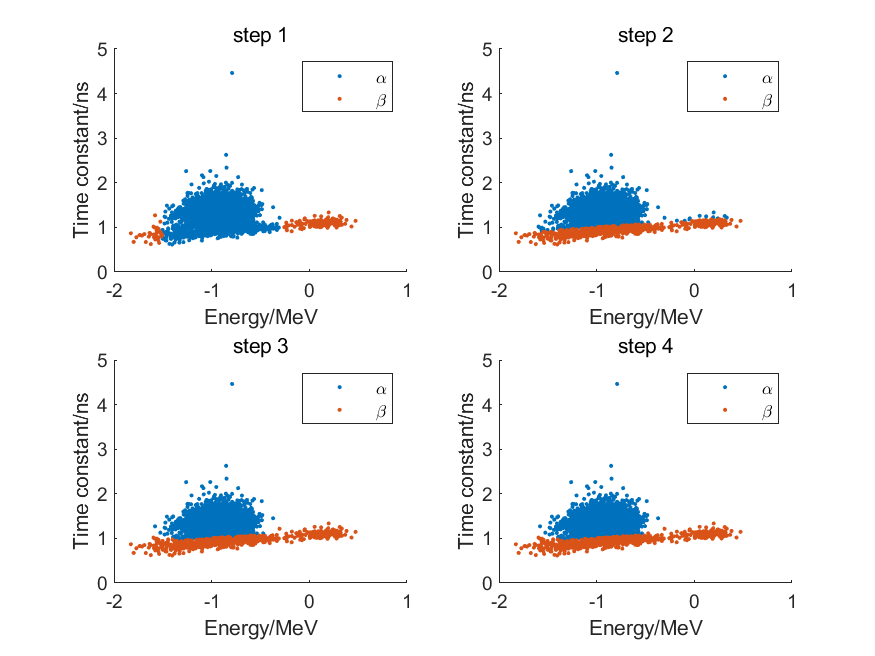
\includegraphics[width=5 in]{figure1.png}
	\caption{The process of how cluster works }
	\label{fig:2}
	\end{figure}
	
	\par step 1. Using projection of energy dimension in log scale, using a normal distribution fitting to find the point beyond 3 $\sigma$, and defined as $\beta$ particle.
	\par step 2. Using a linear fitting to these points, finding the residual less than $+1 \sigma$. 
	\par step 3. Sort out the noise points beyond $3\sigma$ of rest points, by Gaussian fitting. Later classification is based on the minimum distance to the sorted points defined as the same class. 
	\par step 4. Repeat classification by kNN until converge.
	
\section{Simulation and Result}

\subsection{Using JSAP Simulation to provide unlabled data}
\subsubsection{Introduction to JSAP } 
	CJPL is located in Sichuan province with over 2000 meters, CJPL has the lowest cosmic rays and reactor neutrino flux background in the world\\
	JSAP use GEANT LAB + 0.07mg/L PPO and 13ug/L bis-MSB as the reaction material.\\
\subsubsection{Introduction to the detector parameters(table1)}
	The detector radius, PMT response and other detail are shown in table 1.
	parameter of LS material: table 1\\
	
	\begin{table}[h]
	\centering
	\caption{Simulation LS parameters}
	\label{tab:1}
	\begin{tabular}{|l*{1}{l|}}
	\hline
	Parameters & value\\
	\hline
	Detector Radius & 14.5  m\\
	Transit time spread (TTS) & 5.5 ns  \\
	Quantum efficiency & 0.2 \\
	Attenuation length & $\sim$ 18 m\\
	Light yield & 4300/MeV \\
	\hline
	\end{tabular}
	\end{table}
	
\subsubsection{Introduction to the scintillator parameters}
\par Scintillation photons are emitted when the molecule deexcite. and the time scaled by a double decay distribution. 

	\begin{equation}
	\numberwithin{equation}{section}
		p(t) = \frac{\tau_r+\tau_d}{\tau_d^2}\exp(-\frac{t}{\tau_d})(1-\exp(-\frac{t}{\tau_r}))
	\end{equation}
	
\par The decay time constant is relative to the energy, which is useful for energy reconstruction and particle identification. We set a log relationship of the decay time constant and energy. 
\par Parameter of time profile, see figure \ref{fig:3}\\

	\begin{figure}[h]
	\centering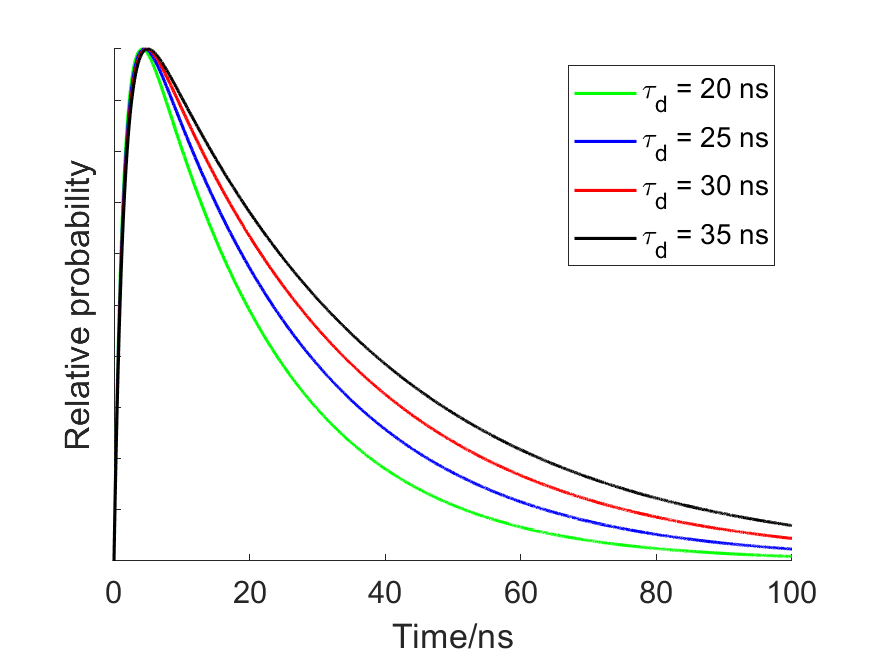
\includegraphics[width=3 in]{time_profile.png}
	\caption{Time profile due to different $\tau_d$}
	\label{fig:3}
	\end{figure}
	
\subsection{Unsupervised reconstruction result comparing to simulation truth information}
\subsubsection{How we plot our result and what info will be put on}
\par 1. The best $\Theta^{[k]}$ and $\tau^{[k]}$ will be found until converged. 
\par 2. We divided the detectors into many bins in 2-d to show the results.
\par 3. The resolution is calculated by distance from reconstructed vertex to truth vertex \\ 

\subsubsection{Describe the result by pictures}
And describe the following picture in detail, each paragraph for a detailed description.
\par 1. Performance of single class reconstruction
\par table1:
	\begin{table}[htbp]
		\centering
		\caption{Simulation LS parameters 0-th iteration}
		\label{tab:4}	
		\begin{tabular}{|r|*{3}{r|}}
		\hline
		Uncertainty & sci & sci + che & sci + che + noise\\
		\hline
		0.2 MeV(center)/m & 0 & 0 & 0 \\
		1 MeV(center)/m & 0 & 0 & 0 \\
		2 MeV(center)/m & 0 & 0 & 0 \\
		\hline
		\end{tabular}
	\end{table}
	
\par picture1: Resolution vs Energy and radius : At different position with energy, the reconstruction result will be ... see figure \ref{fig:4}
\par picture2: Reconstruct time profile vs real profile : The reconstructed time profile comparing to the real profile will be ...
\par picture3: Resolution improvement with or without EM : The resolution changed with iteration will be... (0-th iteration is without EM) see figure \ref{fig:4.3} and figure \ref{fig:4.4}
\begin{figure}[htbp]
\centering

\subfigure[pic1.]{
\begin{minipage}[t]{0.5\linewidth}
\centering
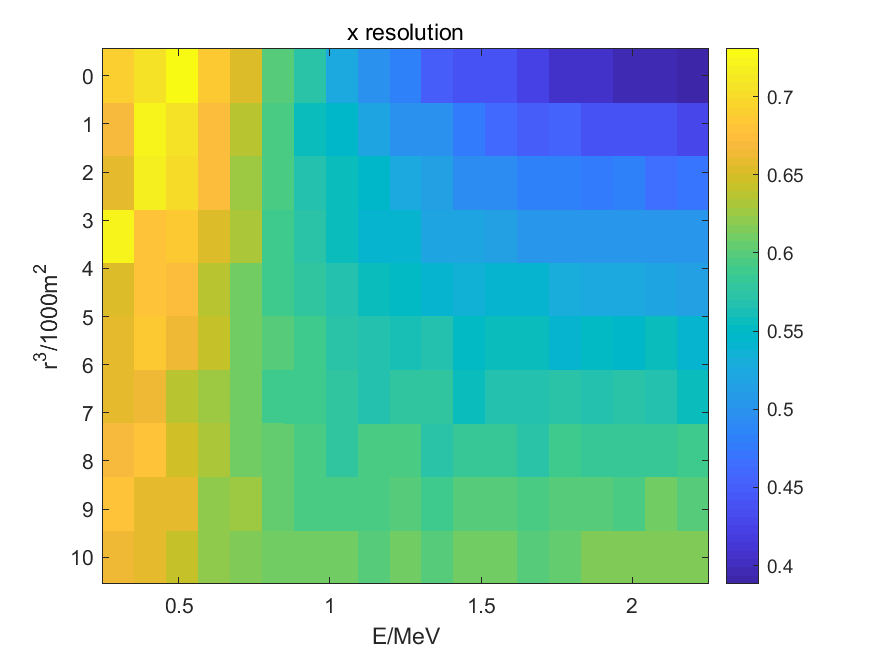
\includegraphics[width=2in]{x_res.png}
%\caption{fig1}
\end{minipage}%
}%
\subfigure[pic2.]{
\begin{minipage}[t]{0.5\linewidth}
\centering
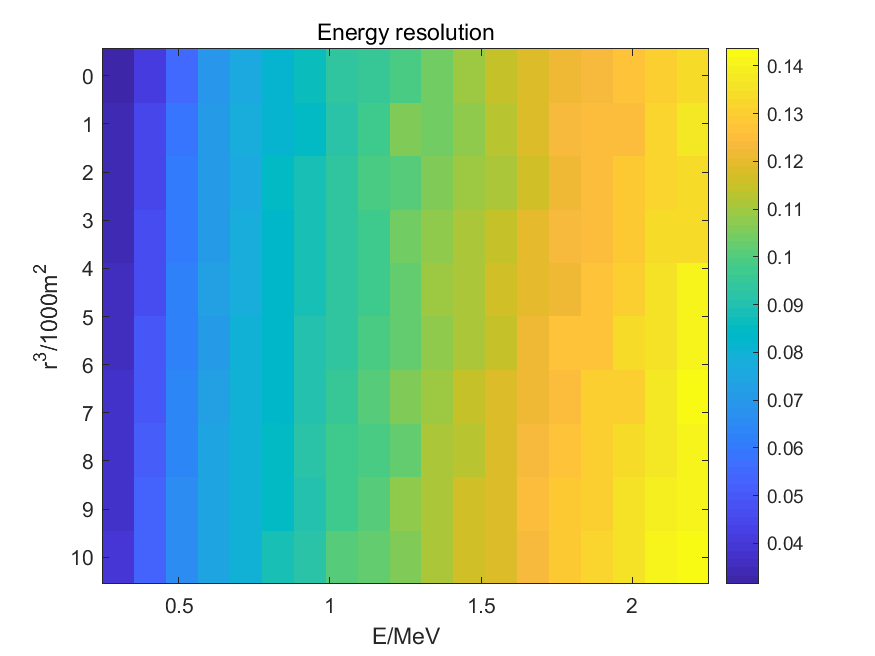
\includegraphics[width=2in]{E_res.png}
%\caption{fig2}
\end{minipage}%
}%


\subfigure[pic3.]{
\begin{minipage}[t]{0.5\linewidth}
\centering
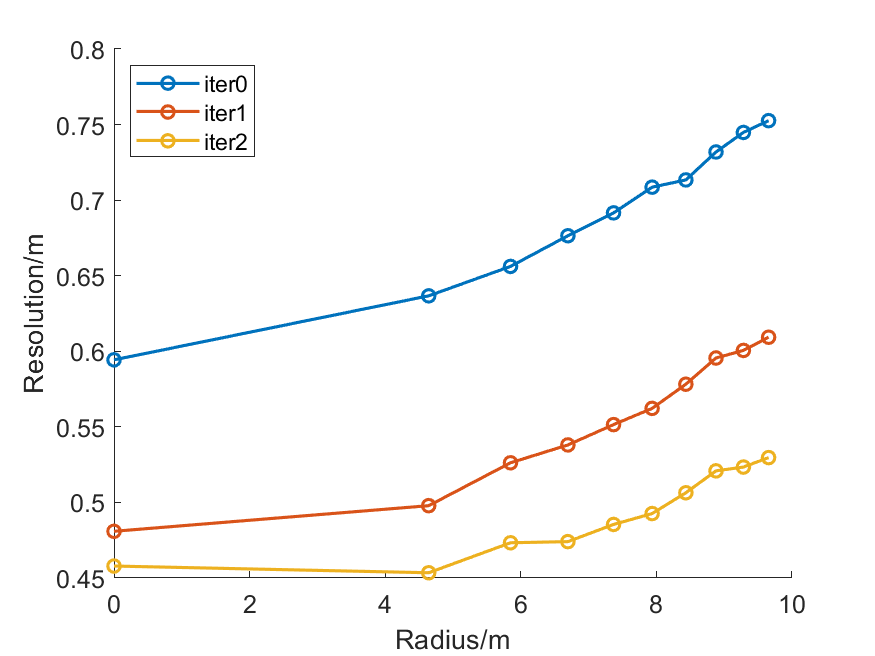
\includegraphics[width=2.2in]{iter1.png}
\label{fig:4.3}
%\caption{fig1}
\end{minipage}%
}%
\subfigure[pic4.]{
\begin{minipage}[t]{0.5\linewidth}
\centering
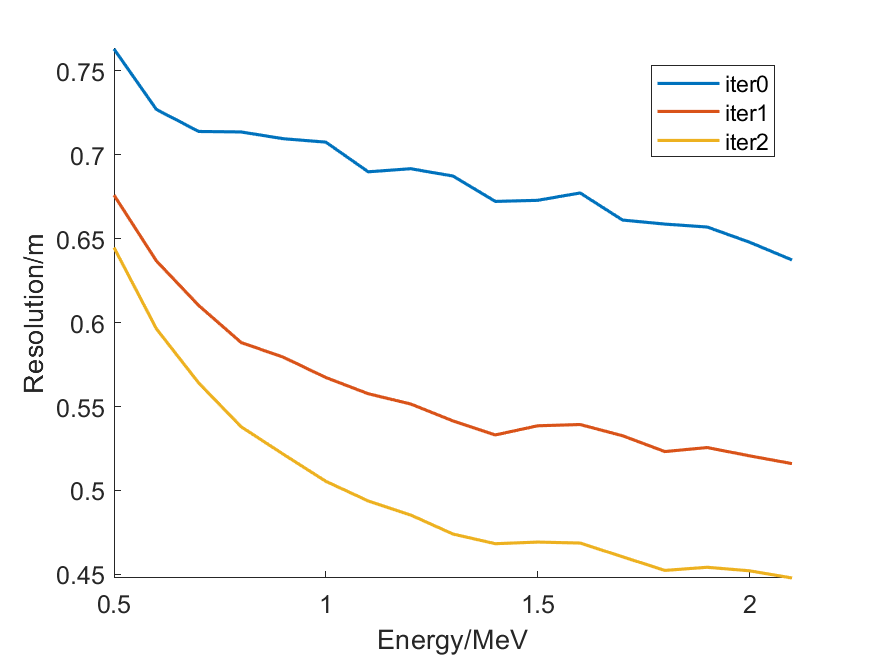
\includegraphics[width=2.2in]{iter2.png}
\label{fig:4.4}
%\caption{fig2}
\end{minipage}%
}%

\subfigure[pic5.]{
\begin{minipage}[t]{0.5\linewidth}
\centering
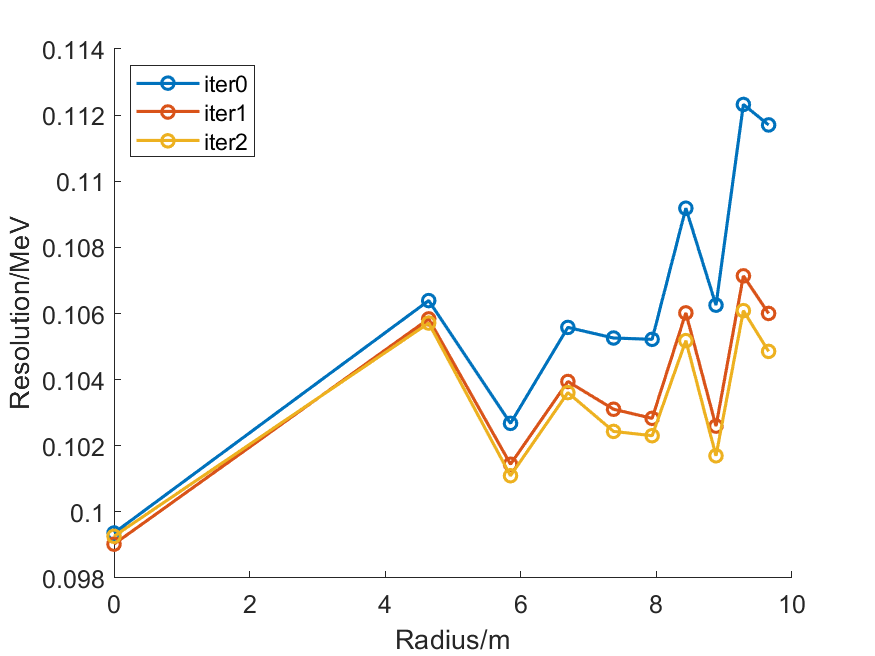
\includegraphics[width=2in]{iter3.png}
%\caption{fig2}
\end{minipage}
}%
\subfigure[pic6.]{
\begin{minipage}[t]{0.5\linewidth}
\centering
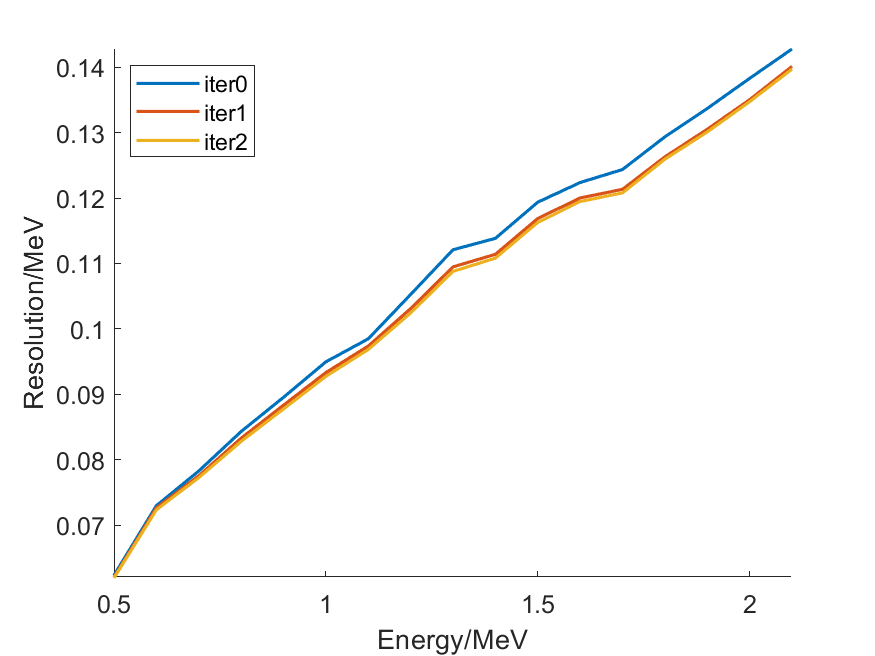
\includegraphics[width=2in]{iter4.png}
%\caption{fig2}
\end{minipage}
}%
\centering
\caption{ Reconstruction of energy and vertex}
\label{fig:4}
\end{figure}

\par 2. Performance of double classes reconstruction
\par table 1:
	\begin{table}[htbp]
		\centering
		\caption{Simulation LS parameters 0-th iteration}
		\label{tab:4}	
		\begin{tabular}{|r|*{3}{r|}}
		\hline
		Uncertainty & sci & sci + Che & sci + Che + noise\\
		\hline
		0.2 MeV(center)/m & 0 & 0 & 0 \\
		1 MeV(center)/m & 0 & 0 & 0 \\
		2 MeV(center)/m & 0 & 0 & 0 \\
		\hline
		\end{tabular}
	\end{table}
	
\par picture1: Resolution vs Energy and radius : At different position with energy, the reconstruction result will be ...
\par picture2: Reconstructed time profile vs real profile : The reconstructed time profile comparing to the real profile will be ...
\par picture3: Resolution improvement with or without EM : The resolution changed with iteration will be... (0-th iteration is without EM)
\subsection{Process the data} 
\subsubsection{Particle identification}
\par A cluster can applied to separate particles. The cluster is following the 4 steps.
\par According to the result, the 2 particles can be classified by given the probability of each class. The error rate is then shown in table.
\subsubsection{Energy dependent time profile}
\par Decay time constant relative to energy can be plot by piece-wise function.

\section{Conclusion and Discussion}
\subsection{Some impressive results in the picture}
1. whether it is effective to single class reconstruction. 2. whether it is effective to double classes reconstruction 3. the performance comparing to the situation with noise or Cherenkov. \\
\subsection{The reached resolution comparing to the traditional method}
1. The reached resolution comparing to the theoretical. 2. The reached resolution comparing to the other experiment.\\
\subsection{What can be done in the future}
1. optics and geometry may be needed. \\

\section{Appendix}
\subsection{Resolution derivation}
\subsection{Initial guess}
\end{document}